%%% TIPO DE DOCUMENTO 

\documentclass{beamer}

\usetheme{Madrid}
\usecolortheme{seagull}
\usefonttheme{professionalfonts}

\useoutertheme{infolines}

%%% IMPORTAMOS PAQUETES A USAR 

\usepackage[utf8]{inputenc}
%\usepackage[latin1]{inputenc}
\usepackage[spanish, es-tabla]{babel}
\usepackage{csquotes}
\usepackage{float}
\usepackage{bbding}
\usepackage{graphicx}
\usepackage{hyperref}
%Pruebas para animaciones
\usepackage{animate}
\usepackage[document]{ragged2e}
\usepackage{bibentry}
\usepackage{graphicx} % Allows including images
\usepackage{booktabs} % Allows the use of \toprule, 
%%%START APA
\usepackage{multicol}
%\usepackage[british]{babel}
%\usepackage[backend=biber,style=apa]{biblatex} OJO CON ESTA LINEA
\setbeamertemplate{navigation symbols}{} % To remove the navigation symbols from the bottom of all slides uncomment this line
%\DeclareLanguageMapping{british}{british-apa}
%\addbibresource{references.bib}
%% APA citing
%% \cite{t} - Uthor und Richter, 2010
%% \textcite{t} - Uthor und Riter (2010)
%% \parencite{t} - (Uthor & Riter, 2010)
%% \parencite[Chapt.~4]{t} - (Uthor & Riter, 2010, S. 15)
%%%END APA

%%%%% =================  PORTADA ================== 
\setbeamercolor{postit}{bg=gray!30!white}
\title[Git y GitHub] 
{Control de versiones con Git y GitHub }
%\subtitle {ne compléter que si l'article possède un sous-titre}

\author[Expertic] 
%\author[Pedro A. Salgado-Meza ]
{Expertic} %\inst{1} \inst{3}}
%{P. A. ~Salgado-Meza\inst{1} \inst{2}}%\and I.~Borne\inst{1} \and J.~Buisson\inst{2}}

\institute[]{
\inst{}Escuela de Física, Universidad Industrial de Santander, Bucaramanga, Colombia.}
%\institute[]
%{
%  \inst{1}%
%  Universidad Industrial de Santander, Bucaramanga, Colombia
%  \and
%  \inst{2}%
%  Escuela de Ingenierías Eléctrica, Electrónica y Telecomunicaciones
%  \and
%  \inst{3}%
%  Escuela de Ingeniería Mecánica  
%  }

\date{\today}


\begin{document}
\logo{
\includegraphics[scale=0.05]{imagenes/Expertic}} 


\begin{frame}
\titlepage % Print the title page as the first slide
\end{frame}

\begin{frame}{Contenido}
  \tableofcontents
\end{frame}

\section{Control de versiones}
\begin{frame}
\centering

\includegraphics[scale=0.3]{Imagenes/Final_doc} 
\end{frame}

\subsection{¿Qué es el control de versiones?}
\begin{frame}{¿Qué es el control de versiones?}
 \footnotesize
 Es un sistema que registra los cambios en un archivo o conjunto de archivos en el tiempo de manera que podamos obtener     versiones específicas después.  \\ 

 \begin{itemize}
  \item Permite regresar un archivo a su estado anterior. 
  \item Revertir todo el proceso a un estado anterior.
  \item Comparar cambios en el tiempo.
  \item Ver quien modificó un archivo.
 \end{itemize}
 \begin{figure}
  \centering
%\raggedright
  
\includegraphics[scale=0.2]{Imagenes/kermit}
 \end{figure}
\centering
\textbf{Una forma de protegernos de nosotros mismos.}
\end{frame}

\subsection{Control de versiones - \textbf{Local}}
\begin{frame}{Control de versiones - \textbf{Local}}
 \begin{columns}
 \column{.45\textwidth}
\begin{figure}
  \centering
%\raggedright
  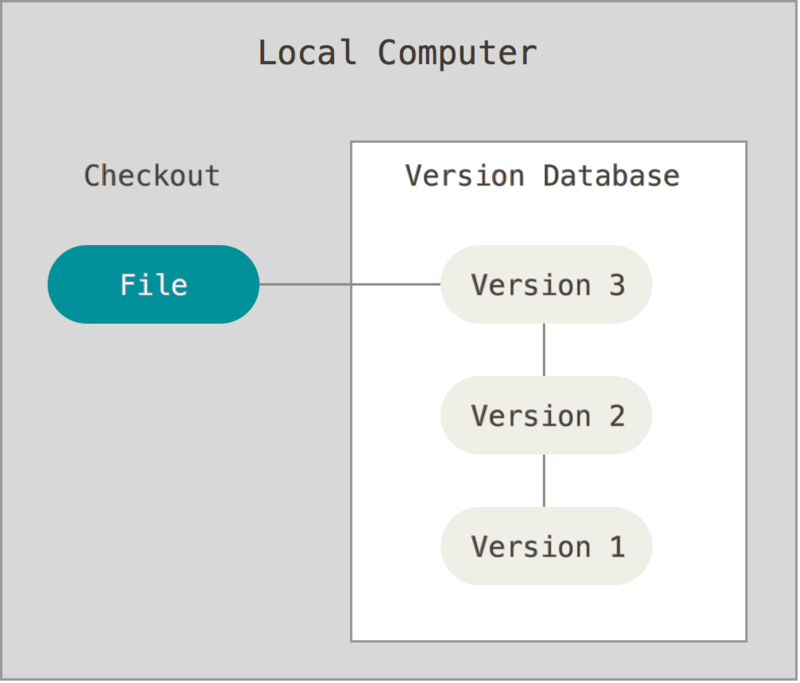
\includegraphics[scale=0.2]{Imagenes/local_vcs}
 \end{figure}

 \column{.45\textwidth}
 \footnotesize
 Son bases de datos locales que guardan todos los archivos bajo control y permiten revertir el estado de estos a una versión anterior.\\
 \vspace{2mm}
 \footnotesize
 El problema es la necesidad de colaborar con otros desarrolladores.
 \end{columns}
\end{frame}

\subsection{Control de versiones - \textbf{Centralizado}}
\begin{frame}{Control de versiones - \textbf{Centralizado}}
 \begin{columns}
 \column{.45\textwidth}
 \begin{figure}
 \centering
%\raggedright
 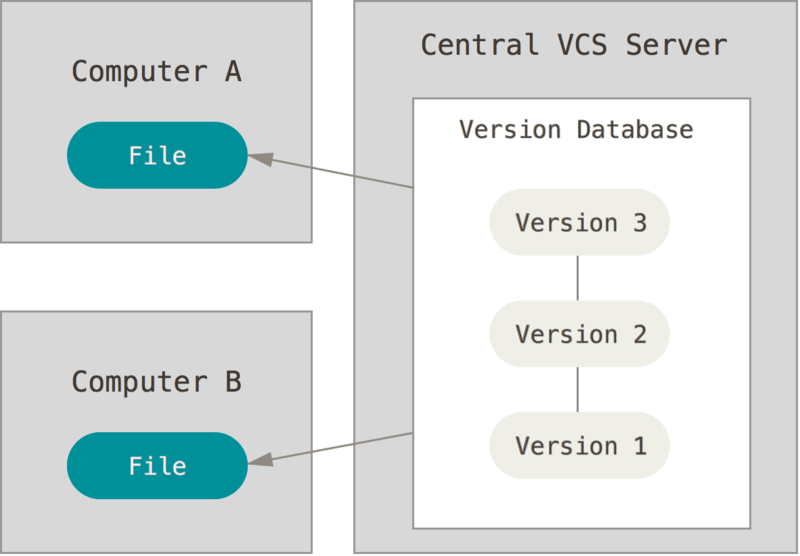
\includegraphics[scale=0.2]{Imagenes/centralized_vcs}
 \end{figure}
 
  \column{.45\textwidth}
  \footnotesize
  Un servidor contiene todos los archivos en diferentes versiones y los clientes sacan la última versión del archivo del sistema central. \\
  \footnotesize
   \vspace{2mm}
  El problema es que al fallar el servidor central durante un tiempo, impide que se pueda colaborar o guardar nuevas versiones.
 \end{columns}
\end{frame}

\subsection{Control de versiones - \textbf{Distribuido}}
\begin{frame}{Control de versiones - \textbf{Distribuido}}
\begin{columns}
 \column{.45\textwidth}
 \begin{figure}
 \centering
%\raggedright
 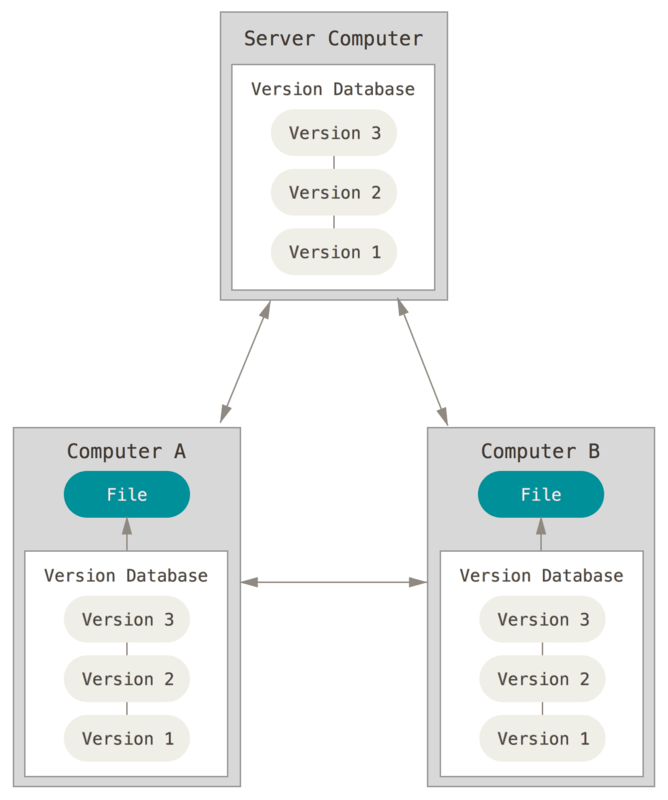
\includegraphics[scale=0.2]{Imagenes/distributed_vcs}
 \end{figure}
 
  \column{.45\textwidth}
  \footnotesize
 En esta versión los clientes no solo sacan la ultima versión, sino que copian todo el repositorio incluyendo el historial de versiones. \textit{Cada copia es un respaldo de todos los datos y se puede usar para restaurarlo de ser necesario.}
 \end{columns}
\end{frame}

\section{Breve historia de Git}
\begin{frame}{Breve historia de Git}
\textbf{Historia}
  \vspace{2mm}
\begin{itemize}
\item Fue creado por \textit{Linus Torvalds} y la comunidad en 2005.
\item Se usó y desarrolló para la creación del kernel de Linux.
\end{itemize}
  \vspace{2mm}
\textbf{Objetivos durante su diseño}
  \vspace{2mm}
\begin{itemize}
\item Velocidad.
\item Diseño simple.
\item Soporte para el desarrollo no lineal (ramas).
\item Capacidad para manejar grandes proyectos.
\end{itemize}
\end{frame}

\section*{Aportes de Git}
\begin{frame}{Aportes de Git}
\begin{itemize}
\item Auditoria completa del código, sabiendo en todo momento quién ha tocado algo, cuándo y qué.
\item Control sobre cómo ha ido cambiando nuestro proyecto con el paso del tiempo.
\item Control de versiones del proyecto por medio de etiquetas.
\item Seguridad e integridad, es imposible modificar archivos sin que Git lo detecte.
\end{itemize}
\end{frame}

\section{Instalación}
\begin{frame}{Instalación}

\textbf{Git desde terminal} \\

\textbf{Linux} \\

Se puede instalar ejecutando desde la terminal \\

\begin{beamercolorbox}[wd={5cm},sep=1mm]{postit}
sudo apt-get install git
\end{beamercolorbox}

\textbf{Windows y Mac} \\

\href{https://git-scm.com/downloads}{\textcolor{blue}{Enlace}} \\

\textbf{Git desde una interfaz}\\
Es posible utilizar Git desde una interfaz gráfica. \\

\href{https://www.gitkraken.com/}{\textcolor{blue}{Kraken}}

\begin{block}
\tiny{
Lo más importante a recordar es que \textbf{Git} es distribuido, por lo que tendremos un repositorio local que vive en un directorio oculto llamado \textbf{.git/} y normalmente (aunque no es obligación) tendremos un remoto, un repositorio central donde diferentes colaboradores puede contribuir.} \\

Notando que cada uno de esos colaboradores tienen una copia exacta de el repositorio en su estación de trabajo.
\end{block}
\end{frame}

\section{Control de versiones - \textbf{Local}}
\subsection{Estados}
\begin{frame}{Control de versiones - \textbf{Local}}
Git tiene tres estados principales donde estarán los archivos: \textit{committed}, \textit{modified} y \textit{staged} \\

\begin{itemize}
\item \textcolor{red}{modificado} (modified) cambia un archivo pero no lo hemos guardado en la base de datos.
\item \textcolor{green}{preparado} (staged) marcamos un archivo modificado en su versión actual para guardarlo en la base de datos.
\item \textcolor{gray}{confirmado}  (committed) los datos están guardados en la base de datos local.
\end{itemize}
\end{frame}

\subsection{Directorios}
\begin{frame}
\begin{columns}
\column{.45\textwidth}
 \begin{figure}
 \centering
%\raggedright
 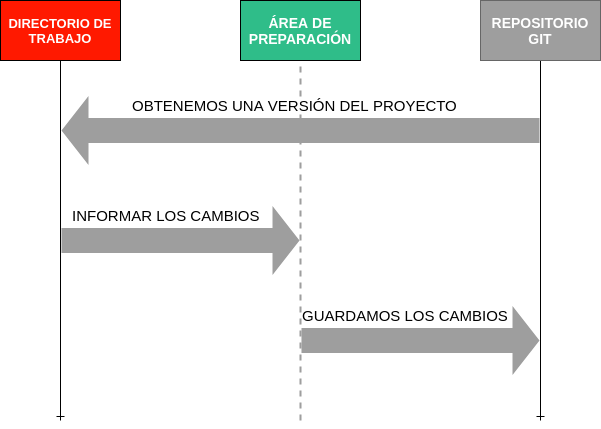
\includegraphics[scale=0.24]{Imagenes/3_states}
 \end{figure}
 \column{.50\textwidth}
    \footnotesize
  \begin{itemize}
  \item \textbf{El directorio de trabajo} es donde estoy trabajando en los archivos, en una versión especifica del proyecto.
  \item \textbf{El área de preparación} es un área virtual, que guarda la información de los cambios que el usuario pretende registrar como una nueva versión.
  \item \textbf{El repositorio Git} es donde Git guarda los metadatos, es decir el registro de los cambios y las versiones del proyecto que se han decidido salvar.
  \end{itemize}
  \end{columns}
\end{frame}

\section{Configuración inicial y ayuda}
\begin{frame}{Configuración inicial y ayuda}
Creamos las credenciales de usuario \\
\begin{beamercolorbox}[sep=1mm]{postit}
git config - -global user.name '' Expertic ''
\end{beamercolorbox}
\begin{beamercolorbox}[sep=1mm]{postit}
git config - -global user.email '' expertic@saber.uis.edu.co ''
\end{beamercolorbox}
Configurar nuestro editor de texto favorito   \\
\begin{beamercolorbox}[sep=1mm]{postit}
git config - -global core.editor gedit
\end{beamercolorbox}

\vspace{5mm}
Podemos obtener ayuda sobre los comandos y los parámetros de Git \\
Muestra todas las opciones que tiene git.\\
\begin{beamercolorbox}[sep=1mm]{postit}
git help  
\end{beamercolorbox}
Muestra ayuda más especifica en cada una de las opciones mostradas anteriormente.\\
\begin{beamercolorbox}[sep=1mm]{postit}
git help opción 
\end{beamercolorbox}
\end{frame}

\section{Trabajando con Git}
\begin{frame}{Trabajando con Git}
\begin{itemize}
\item Inicializamos Git en el directorio con \\
\begin{beamercolorbox}[sep=1mm]{postit}
git init 
\end{beamercolorbox}
\item Consultar el estado actual del repositorio \\
\begin{beamercolorbox}[sep=1mm]{postit}
git status
\end{beamercolorbox}
\item Agregar al área de preparación  \\
\begin{beamercolorbox}[sep=1mm]{postit}
git add \textit{file}
\end{beamercolorbox}
\item Mostrar las diferencias entre el mismo archivo en diferentes versiones. \\
\begin{beamercolorbox}[sep=1mm]{postit}
git diff \textit{file}
\end{beamercolorbox}
\item Guardar los cambios como una nueva versión \\
\begin{beamercolorbox}[sep=1mm]{postit}
git commit 
\end{beamercolorbox}
\end{itemize}
Para profundizar en Git haga clic  \href{https://git-scm.com/book/en/v2}{\textcolor{blue}{Aquí}}
\end{frame}

\section{Trabajando con GitHub}
\begin{frame}{Trabajando con GitHub}
\textbf{¿Qué es GitHub?}\\
Es una plataforma para control de versiones y colaboración. Permite que múltiples personas puedan trabajar en proyectos.\\
\vspace{2mm}
\textbf{Características}
\begin{itemize}
\item Múltiples empresas y universidades comparten sus desarrollos.
\item Es totalmente gratis siempre y cuando el acceso sea público.
\item Podemos subir cualquier tipo de elementos, no sólo código.
\item Podemos conocer las mejores prácticas en cualquier lenguaje.
\end{itemize}

Crear una cuenta \href{www.github.com}{\textcolor{blue}{Aquí}}
\end{frame}

\begin{frame}
\begin{itemize}
\item  Para comunicarnos con Github debemos configurar el repositorio externo, un remoto al que llamamos origin para que podamos subir los cambios. 
\begin{beamercolorbox}[sep=1mm]{postit}
git remote add origin URL-REPO
\end{beamercolorbox}
\item Este es un comando que dice Suba todos los \textit{commits} en la rama llamada \textit{master} al remoto llamado \textit{origin}.
\begin{beamercolorbox}[sep=1mm]{postit}
git push origin master
\end{beamercolorbox}
\item Es usado para apuntar a un repositorio existente y hacer una copia en un nuevo directorio. Esto copia toda la historia del repositorio, todos los commits y la rama a la que apunta el repo remoto.
\begin{beamercolorbox}[sep=1mm]{postit}
git clone URL-REPO
\end{beamercolorbox}
\item Este comando es usado para descargar el contenido de un repositorio remoto inmediatamente mezclar con el repositorio local para sincronizar el contenido. 
\begin{beamercolorbox}[wd={9cm},sep=1mm]{postit}
git pull
\end{beamercolorbox}
\end{itemize}
\end{frame}

\section{Ramas y Merge}
\subsection{Ramas}
\begin{frame}{Ramas}
A partir de una base común podemos crear ramas para cada nueva funcionalidad, la idea con separar el proyecto en múltiples ramas es encapsular los cambios y hace más difícil que código inestable se mezcle con la rama principal. \\
 \begin{figure}
 \centering
%\raggedright
 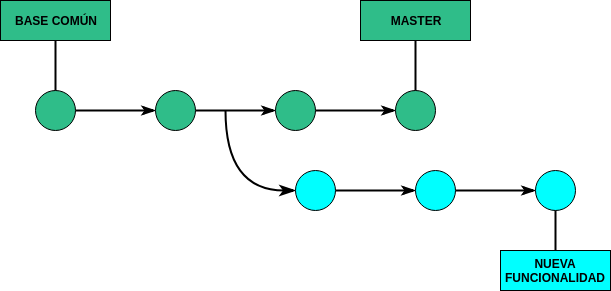
\includegraphics[scale=0.45]{Imagenes/branch}
 \end{figure}
\end{frame}

\subsection{Merge}
\begin{frame}{Merge}
Un merge es la forma de unir la historia de ramas separadas e integrarlas en una sola rama. \\

Git automáticamente une los commits a menos que existan conflictos en ambas ramas.
 \begin{figure}
 \centering
%\raggedright
 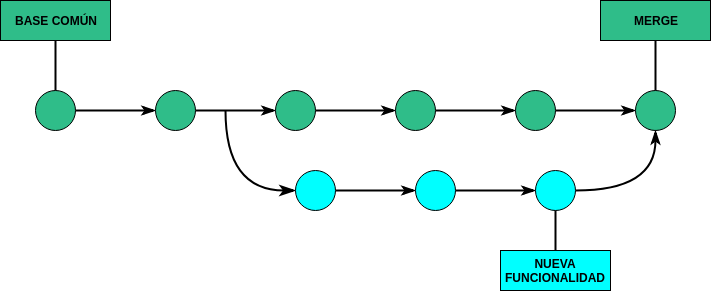
\includegraphics[scale=0.45]{Imagenes/merge}
 \end{figure}
\end{frame}

\begin{frame}
\centering
Gracias...
\end{frame}
\end{document}